\documentclass[12pt,a4paper]{article}
\usepackage[utf8]{inputenc}
\usepackage[T1]{fontenc}
\usepackage{geometry}
\usepackage{listings}
\usepackage{xcolor}
\usepackage{hyperref}
\usepackage{titlesec}
\usepackage{enumitem}
\usepackage{booktabs}
\usepackage{longtable}
\usepackage{array}
\usepackage{fancyhdr}
\usepackage{graphicx}
\usepackage{tikz}
\usetikzlibrary{shapes.geometric, arrows.meta, positioning}

\geometry{margin=2.5cm}

% Colors
\definecolor{codeblue}{RGB}{30,100,200}
\definecolor{codegray}{RGB}{128,128,128}
\definecolor{codegreen}{RGB}{0,150,80}
\definecolor{codepurple}{RGB}{150,0,200}
\definecolor{backcolor}{RGB}{248,248,248}
\definecolor{primaryblue}{RGB}{25,80,160}
\definecolor{accentgreen}{RGB}{0,140,70}

% Code listing style
\lstdefinestyle{bashstyle}{
    backgroundcolor=\color{backcolor},
    commentstyle=\color{codegreen},
    keywordstyle=\color{codeblue}\bfseries,
    stringstyle=\color{codepurple},
    basicstyle=\ttfamily\small,
    breakatwhitespace=false,
    breaklines=true,
    captionpos=b,
    frame=single,
    rulecolor=\color{codegray},
    keepspaces=true,
    numberstyle=\tiny\color{codegray},
    numbers=left,
    showspaces=false,
    showstringspaces=false,
    tabsize=4
}

\lstdefinestyle{sqlstyle}{
    backgroundcolor=\color{backcolor},
    commentstyle=\color{codegreen}\itshape,
    keywordstyle=\color{codeblue}\bfseries,
    stringstyle=\color{codepurple},
    basicstyle=\ttfamily\small,
    morekeywords={SELECT, FROM, WHERE, INSERT, INTO, VALUES, CREATE, OR,
                  REPLACE, FUNCTION, RETURNS, TRIGGER, AS, BEGIN, PERFORM,
                  RETURN, NEW, END, LANGUAGE, PLPGSQL, AFTER, FOR, EACH,
                  ROW, EXECUTE, JOIN, LEFT, DISTINCT, ON, ORDER, BY, DESC,
                  LIMIT, AND, COALESCE, TABLE, PRIMARY, KEY, UNIQUE, NOT,
                  NULL, INTERVAL, NOW, WITH},
    breaklines=true,
    frame=single,
    rulecolor=\color{codegray},
    numbers=left,
    numberstyle=\tiny\color{codegray},
    tabsize=4
}

\lstdefinestyle{pythonstyle}{
    backgroundcolor=\color{backcolor},
    commentstyle=\color{codegreen}\itshape,
    keywordstyle=\color{codeblue}\bfseries,
    stringstyle=\color{codepurple},
    basicstyle=\ttfamily\small,
    morekeywords={def, import, from, return, if, else, elif, True, False,
                  None, while, for, in, try, except, with, class, as},
    breaklines=true,
    frame=single,
    rulecolor=\color{codegray},
    numbers=left,
    numberstyle=\tiny\color{codegray},
    tabsize=4
}

% Header/Footer
\pagestyle{fancy}
\fancyhf{}
\fancyhead[L]{\color{primaryblue}\textbf{Gateway Gulf HRM}}
\fancyhead[R]{\color{codegray}Attendance Sync System}
\fancyfoot[C]{\thepage}
\renewcommand{\headrulewidth}{0.5pt}

% Section formatting
\titleformat{\section}{\Large\bfseries\color{primaryblue}}{{\thesection}}{1em}{}[\titlerule]
\titleformat{\subsection}{\large\bfseries\color{primaryblue}}{\thesubsection}{1em}{}
\titleformat{\subsubsection}{\normalsize\bfseries\color{accentgreen}}{\thesubsubsection}{1em}{}

\hypersetup{
    colorlinks=true,
    linkcolor=primaryblue,
    urlcolor=codeblue,
}

% ─────────────────────────────────────────────────────────────────────────────
\begin{document}

\begin{titlepage}
    \centering
    \vspace*{2cm}
    {\color{primaryblue}\rule{\linewidth}{1.5pt}}\\[0.5cm]
    {\Huge\bfseries\color{primaryblue} Attendance Sync System}\\[0.3cm]
    {\Large\color{codegray} Technical Documentation}\\[0.3cm]
    {\color{primaryblue}\rule{\linewidth}{1.5pt}}\\[1.5cm]
    {\large\textbf{Project:} Gateway Gulf HRM}\\[0.3cm]
    {\large\textbf{Version:} 2.0}\\[0.3cm]
    {\large\textbf{Date:} August 2026}\\[0.3cm]
    {\large\textbf{Author:} S-Byte / Sanadi Technologies}\\[2cm]
    \vfill
    {\color{codegray}\small This document covers the real-time biometric attendance sync
    architecture, deployment steps, and operational guide for the Gateway Gulf HRM system.}
\end{titlepage}

\tableofcontents
\newpage

% ─────────────────────────────────────────────────────────────────────────────
\section{Overview}

The Attendance Sync System provides real-time synchronisation between the
BioTime biometric device database (\texttt{GATEWAY\_BIOTIME\_SYNC}) and the
HRM attendance database (\texttt{gateway\_gulf\_prod}). It replaces the
previous batch-scheduled approach with an event-driven architecture using
PostgreSQL \texttt{LISTEN/NOTIFY}.

\subsection{Key Features}

\begin{itemize}[leftmargin=2em]
    \item \textbf{Real-time sync} — attendance updated within seconds of a
          biometric punch
    \item \textbf{Zero idle load} — daemon sleeps until a punch arrives;
          no polling
    \item \textbf{Offline device resilience} — devices that reconnect after
          being offline push all queued punches; all are processed correctly
    \item \textbf{Daemon crash recovery} — watermark file tracks the last
          processed timestamp; catchup runs automatically on restart
    \item \textbf{Manual backfill} — existing management command for
          date-range and per-employee reprocessing
    \item \textbf{Calendar/Working day leave logic} — leave status respects
          \texttt{type\_of\_days} from the leave policy
\end{itemize}

% ─────────────────────────────────────────────────────────────────────────────
\section{Architecture}

\subsection{System Flow}

\begin{center}
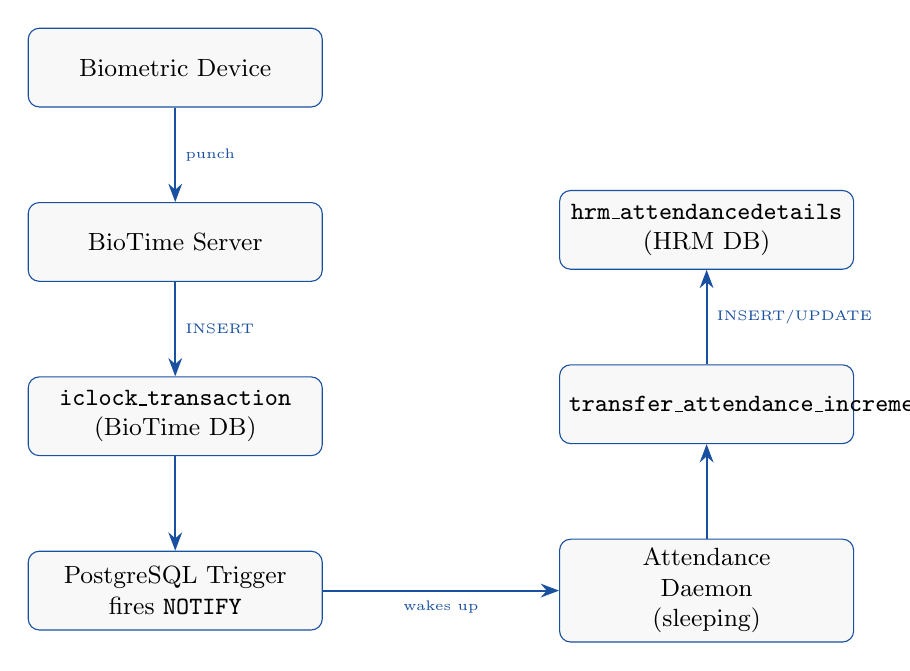
\begin{tikzpicture}[
    node distance=1.2cm and 2cm,
    box/.style={rectangle, rounded corners=4pt, draw=primaryblue,
                fill=backcolor, text width=3.5cm, align=center,
                minimum height=1cm, font=\small},
    arrow/.style={-{Stealth}, thick, color=primaryblue}
]
\node[box] (device)   {Biometric Device};
\node[box] (biotime)  [below=of device]  {BioTime Server};
\node[box] (iclock)   [below=of biotime] {\texttt{iclock\_transaction}\\(BioTime DB)};
\node[box] (trigger)  [below=of iclock]  {PostgreSQL Trigger\\fires \texttt{NOTIFY}};
\node[box] (daemon)   [right=3cm of trigger] {Attendance\\Daemon\\(sleeping)};
\node[box] (incremental) [above=of daemon] {\texttt{transfer\_attendance\_incremental()}};
\node[box] (hrm)      [above=of incremental] {\texttt{hrm\_attendancedetails}\\(HRM DB)};

\draw[arrow] (device) -- (biotime) node[midway,right,font=\tiny] {punch};
\draw[arrow] (biotime) -- (iclock) node[midway,right,font=\tiny] {INSERT};
\draw[arrow] (iclock) -- (trigger);
\draw[arrow] (trigger) -- (daemon) node[midway,below,font=\tiny] {wakes up};
\draw[arrow] (daemon) -- (incremental);
\draw[arrow] (incremental) -- (hrm) node[midway,right,font=\tiny] {INSERT/UPDATE};
\end{tikzpicture}
\end{center}

\subsection{File Structure}

\begin{longtable}{>{\ttfamily}p{7.5cm} p{7cm}}
\toprule
\textbf{File} & \textbf{Purpose} \\
\midrule
\endhead
attendance\_scheduler\_tasks/device\_attendance\_task.py
    & Core sync logic — full backfill and incremental sync \\[4pt]
attendance\_scheduler\_tasks/device\_attendance\_daemon.py
    & Daemon — listens on NOTIFY, manages watermark file \\[4pt]
attendance\_scheduler\_tasks/attendance\_daemon.service
    & systemd service unit file \\[4pt]
hrm/management/commands/device\_attendance.py
    & Django management command for manual backfill \\
\bottomrule
\end{longtable}

% ─────────────────────────────────────────────────────────────────────────────
\section{Database Setup}

\subsection{PostgreSQL Trigger (BioTime DB)}

Run once on the \texttt{GATEWAY\_BIOTIME\_SYNC} database:

\begin{lstlisting}[style=sqlstyle, caption={Create notify trigger on iclock\_transaction}]
CREATE OR REPLACE FUNCTION notify_new_punch()
RETURNS trigger AS $$
BEGIN
    PERFORM pg_notify('new_punch', NEW.emp_code::text);
    RETURN NEW;
END;
$$ LANGUAGE plpgsql;

CREATE TRIGGER punch_inserted
AFTER INSERT ON public.iclock_transaction
FOR EACH ROW
EXECUTE FUNCTION notify_new_punch();
\end{lstlisting}

\textbf{Verify trigger was created:}

\begin{lstlisting}[style=sqlstyle, caption={Verify trigger}]
SELECT trigger_name, event_manipulation, event_object_table
FROM information_schema.triggers
WHERE event_object_table = 'iclock_transaction';

-- Manual test (daemon should wake up immediately)
SELECT pg_notify('new_punch', 'test');
\end{lstlisting}

% ─────────────────────────────────────────────────────────────────────────────
\section{Server Deployment}

\subsection{Step 1 — Edit Service File}

\begin{lstlisting}[style=bashstyle, caption={Edit paths in service file}]
nano /etc/systemd/system/attendance_daemon.service
\end{lstlisting}

Update the following two lines with your actual server paths:

\begin{lstlisting}[style=bashstyle, caption={attendance\_daemon.service}]
[Unit]
Description=Attendance Sync Daemon
After=network.target postgresql.service
Wants=postgresql.service

[Service]
Type=simple
User=www-data
WorkingDirectory=/var/www/gateway_hrm/backend
ExecStart=/var/www/gateway_hrm/venv/bin/python \
    attendance_scheduler_tasks/device_attendance_daemon.py
Restart=always
RestartSec=10
StandardOutput=journal
StandardError=journal

[Install]
WantedBy=multi-user.target
\end{lstlisting}

\subsection{Step 2 — Deploy and Start}

\begin{lstlisting}[style=bashstyle, caption={Deploy the systemd service}]
# Copy service file
sudo cp /var/www/gateway_hrm/backend/attendance_scheduler_tasks/ \
        attendance_daemon.service \
        /etc/systemd/system/

# Reload systemd and enable
sudo systemctl daemon-reload
sudo systemctl enable attendance_daemon
sudo systemctl start attendance_daemon
\end{lstlisting}

\subsection{Step 3 — Verify}

\begin{lstlisting}[style=bashstyle, caption={Check daemon status}]
sudo systemctl status attendance_daemon
# Expected: Active: active (running)

# Watch live logs
tail -f /var/www/gateway_hrm/backend/attendance_logs/attendance_daemon.log
\end{lstlisting}

\subsection{Step 4 — Test}

Insert a test punch in the BioTime DB and watch the daemon log:

\begin{lstlisting}[style=sqlstyle, caption={Test punch insert}]
INSERT INTO public.iclock_transaction
(id, emp_code, punch_time, punch_state, verify_type, work_code,
 terminal_sn, terminal_alias, area_alias, longitude, latitude,
 gps_location, mobile, source, purpose, crc, is_attendance,
 reserved, upload_time, sync_status, sync_time, is_mask,
 temperature, emp_id, terminal_id, company_code)
VALUES(
    (SELECT MAX(id) + 1 FROM public.iclock_transaction),
    'E10090', NOW(), '255', '1', '', 'd65775f15b47db27',
    'mobile punch', '', 0.0, 0.0, '', '', 0, 0, '',
    1, '', NOW(), 0, NULL, 0, 0, 48, 0, ''
);
\end{lstlisting}

Expected log output:
\begin{lstlisting}[style=bashstyle]
Notification received - running incremental sync...
Incremental sync complete.
\end{lstlisting}

% ─────────────────────────────────────────────────────────────────────────────
\section{Daemon Behaviour}

\subsection{Normal Operation}

\begin{enumerate}[leftmargin=2em]
    \item Daemon starts and reads \texttt{attendance\_watermark.txt}
    \item If watermark exists, runs a catchup sync for all punches since
          that timestamp
    \item Connects to BioTime DB and issues \texttt{LISTEN new\_punch}
    \item Sleeps inside \texttt{select()} — zero CPU, zero DB queries
    \item On \texttt{NOTIFY}, wakes up and calls
          \texttt{transfer\_attendance\_incremental()}
    \item After sync, updates watermark file with \texttt{max(upload\_time)}
    \item Returns to sleep
\end{enumerate}

\subsection{Resilience Scenarios}

\begin{longtable}{p{4.5cm} p{9cm}}
\toprule
\textbf{Scenario} & \textbf{How it is handled} \\
\midrule
\endhead
Device offline N days, reconnects
    & BioTime pushes all queued punches with \texttt{upload\_time = NOW}.
      Daemon wakes, fetches all rows where \texttt{upload\_time > watermark},
      processes the correct past \texttt{punch\_time} dates. \\[6pt]
Daemon stopped / crashed
    & On restart, reads watermark file, fetches all punches since that
      timestamp, processes the full gap, then resumes listening. \\[6pt]
Server down N days
    & Same as daemon stopped — BioTime queues locally, pushes on reconnect,
      daemon catches up via watermark. \\[6pt]
No new punches
    & Daemon sleeps in \texttt{select()} — zero load on server. \\[6pt]
Daemon crashes
    & systemd restarts it within 10 seconds automatically. \\
\bottomrule
\end{longtable}

\subsection{Watermark File}

The watermark is stored at:
\begin{lstlisting}[style=bashstyle]
backend/attendance_logs/attendance_watermark.txt
\end{lstlisting}

It contains an ISO-format UTC timestamp, e.g.:
\begin{lstlisting}[style=bashstyle]
2026-08-04T10:32:15.123456+00:00
\end{lstlisting}

\textbf{Do not delete this file} unless you want the next run to start
fresh from the last hour only.

% ─────────────────────────────────────────────────────────────────────────────
\section{Manual Backfill Command}

Use the management command for historical reprocessing:

\begin{lstlisting}[style=bashstyle, caption={Management command usage}]
# Full sync for a date range (all employees)
python manage.py device_attendance 2026-07-01 2026-07-31

# Single employee
python manage.py device_attendance 2026-07-01 2026-07-31 \
    --employees E10090

# Multiple employees (comma-separated)
python manage.py device_attendance 2026-07-01 2026-07-31 \
    --employees E10090,E10007,E10179
\end{lstlisting}

\textbf{Note:} The backfill command does not affect the watermark file.
It is independent of the daemon.

% ─────────────────────────────────────────────────────────────────────────────
\section{Leave Type of Days Logic}

Attendance status during leave depends on the \texttt{type\_of\_days}
setting in the \texttt{LeavePolicy} model.

\begin{longtable}{p{3.5cm} p{3cm} p{6cm}}
\toprule
\textbf{Leave Source} & \textbf{type\_of\_days} & \textbf{Behaviour} \\
\midrule
\endhead
Leave Entry & \texttt{Calendar\_days}
    & Leave status applied even on weekly off / holiday \\[4pt]
Leave Entry & \texttt{Working\_days}
    & Weekly off / holiday status takes priority \\[4pt]
Leave Application & \texttt{Calendar\_days}
    & Leave status applied even on weekly off / holiday \\[4pt]
Leave Application & \texttt{Working\_days}
    & Weekly off / holiday status takes priority \\
\bottomrule
\end{longtable}

\texttt{type\_of\_days} for leave applications is resolved from:
\[
\texttt{master\_leaveapplication}
\rightarrow \texttt{master\_leavemasterdetails (latest by id)}
\rightarrow \texttt{master\_leavepolicy.type\_of\_days}
\]

% ─────────────────────────────────────────────────────────────────────────────
\section{Performance Optimisations}

The sync task was rewritten from a per-iteration DB query pattern to a
bulk pre-load pattern. The following table summarises the improvement:

\begin{longtable}{p{5.5cm} p{2.5cm} p{5.5cm}}
\toprule
\textbf{Operation} & \textbf{Before} & \textbf{After} \\
\midrule
\endhead
Bio punch fetch & N×M queries & 1 bulk query \\
Existing attendance check & N×M queries & 1 bulk query \\
Leave entry lookup & N×M queries & 1 bulk query \\
Leave application lookup & N×M queries & 1 bulk query \\
Holiday check & 1 query per call & Pre-loaded list \\
Weekly off parse & JSON parse per date & Once per employee \\
Grace details & DB query per profile & Lazy in-memory cache \\
Shift details & DB query per employee & 1 bulk query \\
\bottomrule
\end{longtable}

\textbf{Result:} Processing 456 employees × 31 days reduced from
\textasciitilde18,000 DB round trips to 6 bulk queries.

% ─────────────────────────────────────────────────────────────────────────────
\section{Daemon Management Commands}

\begin{lstlisting}[style=bashstyle, caption={Common systemctl commands}]
# Start
sudo systemctl start attendance_daemon

# Stop
sudo systemctl stop attendance_daemon

# Restart
sudo systemctl restart attendance_daemon

# Check status
sudo systemctl status attendance_daemon

# View logs (systemd journal)
sudo journalctl -u attendance_daemon -f

# View application logs
tail -f /var/www/gateway_hrm/backend/attendance_logs/attendance_daemon.log
\end{lstlisting}

% ─────────────────────────────────────────────────────────────────────────────
\section{Environment Variables}

The following must be set in \texttt{backend/.env}:

\begin{longtable}{>{\ttfamily}p{5cm} p{8cm}}
\toprule
\textbf{Variable} & \textbf{Description} \\
\midrule
\endhead
DB\_NAME        & HRM PostgreSQL database name \\
DB\_USERNAME    & HRM DB username \\
DB\_PASSWORD    & HRM DB password \\
DB\_SERVER      & HRM DB host \\
DB\_PORT        & HRM DB port (default 5432) \\
DB\_BIO\_NAME   & BioTime DB name \\
DB\_BIO\_USERNAME & BioTime DB username \\
DB\_BIO\_PASSWORD & BioTime DB password \\
DB\_BIO\_SERVER & BioTime DB host \\
DB\_BIO\_PORT   & BioTime DB port (default 5432) \\
\bottomrule
\end{longtable}

% ─────────────────────────────────────────────────────────────────────────────
\section{Troubleshooting}

\begin{longtable}{p{5cm} p{8.5cm}}
\toprule
\textbf{Issue} & \textbf{Fix} \\
\midrule
\endhead
Daemon not waking on punch
    & Verify trigger exists: \texttt{SELECT trigger\_name FROM
      information\_schema.triggers WHERE event\_object\_table =
      'iclock\_transaction';} \\[6pt]
Attendance not updating
    & Check \texttt{is\_attendance = 1} on the punch row and verify
      \texttt{emp\_code} matches an HRM employee \\[6pt]
Watermark file missing
    & First run seeds watermark to \texttt{NOW()}; future punches
      will be caught normally \\[6pt]
Daemon not starting
    & Run \texttt{sudo journalctl -u attendance\_daemon -n 50} to
      see the error \\[6pt]
Leave status not applying
    & Check \texttt{type\_of\_days} on the LeavePolicy for that
      leave type \\
\bottomrule
\end{longtable}

\end{document}
